\documentclass{article}
\usepackage[utf8]{inputenc}
\usepackage{amsmath}
\usepackage{graphicx}
\usepackage{tabularx}
\usepackage{xcolor}
\usepackage{tabularray}
\usepackage{float}
\usepackage{bm}
\usepackage[colorlinks]{hyperref}
\usepackage[normalem]{ulem}
\usepackage[affil-it]{authblk}
\setlength{\parindent}{0pt}
\usepackage{caption}
\captionsetup[table]{position=bottom} 
%\usepackage{draftwatermark}
%\SetWatermarkText{Draft}
%\SetWatermarkScale{4}
%\SetWatermarkColor[gray]{0.97}

\usepackage{titlesec}

\setcounter{secnumdepth}{4}

\titleformat{\paragraph}
{\normalfont\normalsize\bfseries}{\theparagraph}{1em}{}
\titlespacing*{\paragraph}
{0pt}{3.25ex plus 1ex minus .2ex}{1.5ex plus .2ex}

\title{Analysis of UN Actors in the PA-X Agreement-Actor Signatories Dataset}
\author{Roy Gardner}

\begin{document}

\newcolumntype{R}{>{\raggedleft\arraybackslash}X}

\maketitle

\tableofcontents
\newpage

\section{Introduction}

\subsection{Data sources}
The analysis is based on the following signatory data files supplied by Niamh Henry on 03/11/2023:

\begin{itemize}
\item links\_table.csv
\item node\_table.csv
\end{itemize}

\subsection{Search criteria}

The search criteria for UN actors are as follows:

\begin{itemize}
\item The actor \texttt{node\_id} value must start with 'IGO\_' or 'COA\_'.
\item The actor \texttt{node\_name} value must contain 'United Nations' or ' UN', or start with 'UN'.
\end{itemize}

\subsection{Data integrity}

There are unresolved data integrity issues. For example, the analysis described here finds that United Nations (General) (IGO\_49) is a signatory to 272 agreements. However, a search in links\_table.csv for  finds 313 rows containing IGO\_49 in the  \texttt{to\_node\_id} field. \newline

The anomaly is caused by duplicate row in links\_table.csv. For example, rows with \texttt{signatory\_id} values \texttt{1290} and \texttt{1292} are identical in all other fields.\newline


\section{Preliminaries}

\subsection{List of UN Actors}

\begin{table}[H]
\begin{center}
\small
\begin{tabularx}{\textwidth}{|X|l|}
    \hline
    \textbf{Name} & \textbf{Identifier} \\
    \hline
    \hline
        Group of Friends UNSG & COA\_51 \\
	\hline
	Office of the United Nations High Commissioner for Human Rights & IGO\_640 \\
	\hline
	UN General Assembly & IGO\_315 \\
	\hline
	UN Office on Drugs and Crimes & IGO\_672 \\
	\hline
	UN Secretary General & IGO\_386 \\
	\hline
	UN Security Council & IGO\_8 \\
	\hline
	UNAMID & IGO\_950 \\
	\hline
	UNAMSIL & IGO\_652 \\
	\hline
	UNCRO & IGO\_795 \\
	\hline
	UNISFA & IGO\_616 \\
	\hline
	UNMIBH & IGO\_405 \\
	\hline
	UNMIS & IGO\_854 \\
	\hline
	UNMISS & IGO\_831 \\
	\hline
	UNMOT & IGO\_454 \\
	\hline
	UNOMB & IGO\_274 \\
	\hline
	UNOMIG & IGO\_480 \\
	\hline
	UNPOS & IGO\_536 \\
	\hline
	UNPROFOR & IGO\_355 \\
	\hline
	UNSMIL & IGO\_750 \\
	\hline
	United Nations (General) & IGO\_49 \\
	\hline
	United Nations Children's Fund & IGO\_459 \\
	\hline
	United Nations Development Programme & IGO\_64 \\
	\hline
	United Nations Educational, Scientific and Cultural Organization & IGO\_678 \\
	\hline
	United Nations Human Rights Council & IGO\_440 \\
	\hline
	United Nations Population Fund & IGO\_674 \\
	\hline
	United Nations Secretariat & IGO\_391 \\
	\hline
\end{tabularx}
\end{center}
\normalsize
\caption{Names and identifiers of 26 UN actors obtained from the PA-X agreement-actor signatories dataset. }
\end{table}

\subsection{Numerical data}

\begin{table}[H]
\begin{center}
\small
\begin{tabularx}{\textwidth}{|X|r|}
    \hline
    \textbf{Variable} & \textbf{Value} \\
    \hline
    \hline
     Number of agreements in dataset & 1642 \\
     \hline
     Number of actors in dataset & 1096 \\
     \hline
     Number of UN actors in dataset (see Table 1 above) & 26 \\
     \hline
     Number of agreements to which one or more UN actors are signatories & 371 \\
     \hline
     Number of non-UN actors that are co-signatories with UN actors  & 510  \\
     \hline
\end{tabularx}
\end{center}
\normalsize
\caption{Basic numerical data.}
\end{table}

\begin{table}[H]
\begin{center}
\small
\begin{tabularx}{\textwidth}{|X|r|}
    \hline
    \textbf{Variable} & \textbf{Value (\%))} \\
    \hline
    \hline
     UN actors as a percentage of all actors  & 2.4  \\
     \hline
     Agreements signed by UN actors as a percentage of all agreements  & 22.6  \\
     \hline
     Non-UN co-signatories as a percentage of all actors & 46.5  \\
     \hline
\end{tabularx}
\end{center}
\normalsize
\caption{Statistical data.}
\end{table}

\subsection{Number of agreements signed by UN actors}


\begin{figure}[H]
\begin{center}
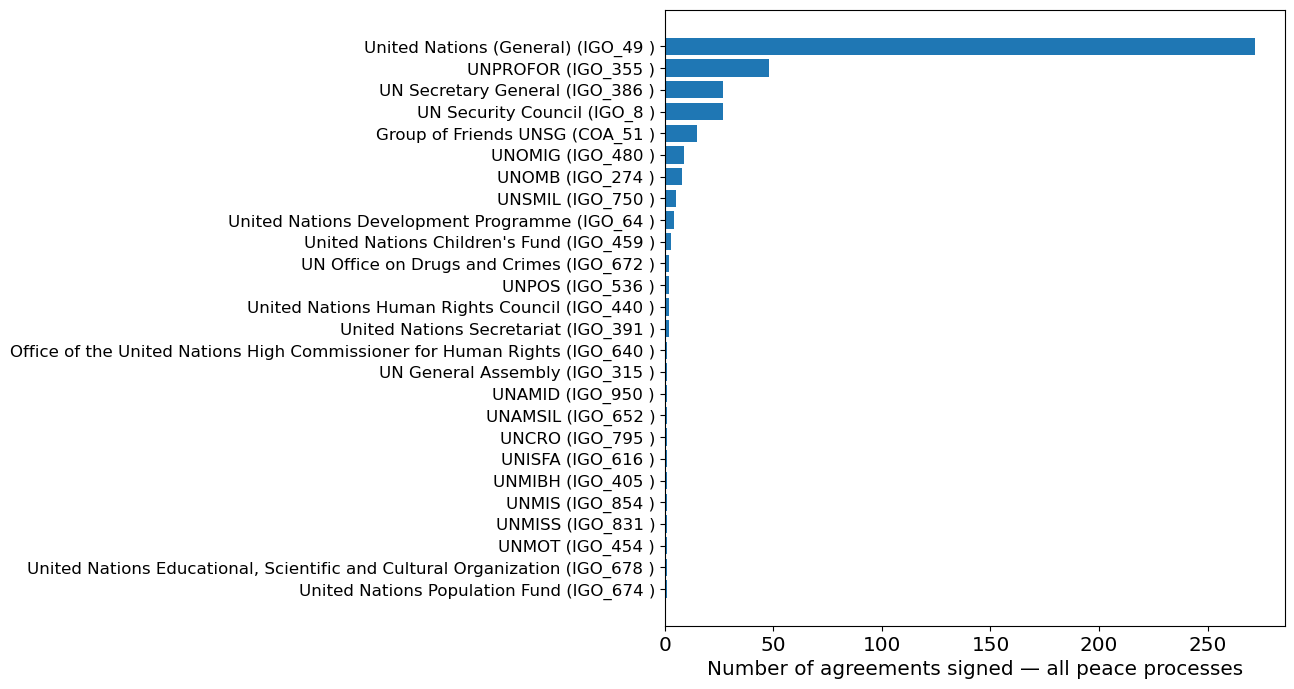
\includegraphics[scale=0.36]{./assets/figure_1.png}
\caption{Number of agreements signed by the 26 UN actors in the analysis. See Table 3 below for exact values.}
\end{center}
\end{figure}

\begin{table}[H]
\begin{center}
\small
\begin{tabularx}{\textwidth}{|X|l|r|}
    \hline
    \textbf{UN actor name} & \textbf{UN actor ID}  & \textbf{Agts} \\
    \hline
    \hline
United Nations (General) & IGO\_49 & 272 \\
\hline
UNPROFOR & IGO\_355 & 48 \\
\hline
UN Secretary General & IGO\_386 & 27 \\
\hline
UN Security Council & IGO\_8 & 27 \\
\hline
Group of Friends UNSG & COA\_51 & 15 \\
\hline
UNOMIG & IGO\_480 & 9 \\
\hline
UNOMB & IGO\_274 & 8 \\
\hline
UNSMIL & IGO\_750 & 5 \\
\hline
United Nations Development Programme & IGO\_64 & 4 \\
\hline
United Nations Children's Fund & IGO\_459 & 3 \\
\hline
UN Office on Drugs and Crimes & IGO\_672 & 2 \\
\hline
UNPOS & IGO\_536 & 2 \\
\hline
United Nations Human Rights Council & IGO\_440 & 2 \\
\hline
United Nations Secretariat & IGO\_391 & 2 \\
\hline
Office of the United Nations High Commissioner for Human Rights & IGO\_640 & 1 \\
\hline
UN General Assembly & IGO\_315 & 1 \\
\hline
UNAMID & IGO\_950 & 1 \\
\hline
UNAMSIL & IGO\_652 & 1 \\
\hline
UNCRO & IGO\_795 & 1 \\
\hline
UNISFA & IGO\_616 & 1 \\
\hline
UNMIBH & IGO\_405 & 1 \\
\hline
UNMIS & IGO\_854 & 1 \\
\hline
UNMISS & IGO\_831 & 1 \\
\hline
UNMOT & IGO\_454 & 1 \\
\hline
United Nations Educational, Scientific and Cultural Organization & IGO\_678 & 1 \\
\hline
United Nations Population Fund & IGO\_674 & 1 \\
\hline
\end{tabularx}
\end{center}
\normalsize
\caption{Number of agreements signed by UN actors in descending order. See Figure 1 above.}
\end{table}

\section{UN Actors Co-signatory Analysis}

\subsection{UN--UN co-signatories}

\begin{figure}[H]
\begin{center}
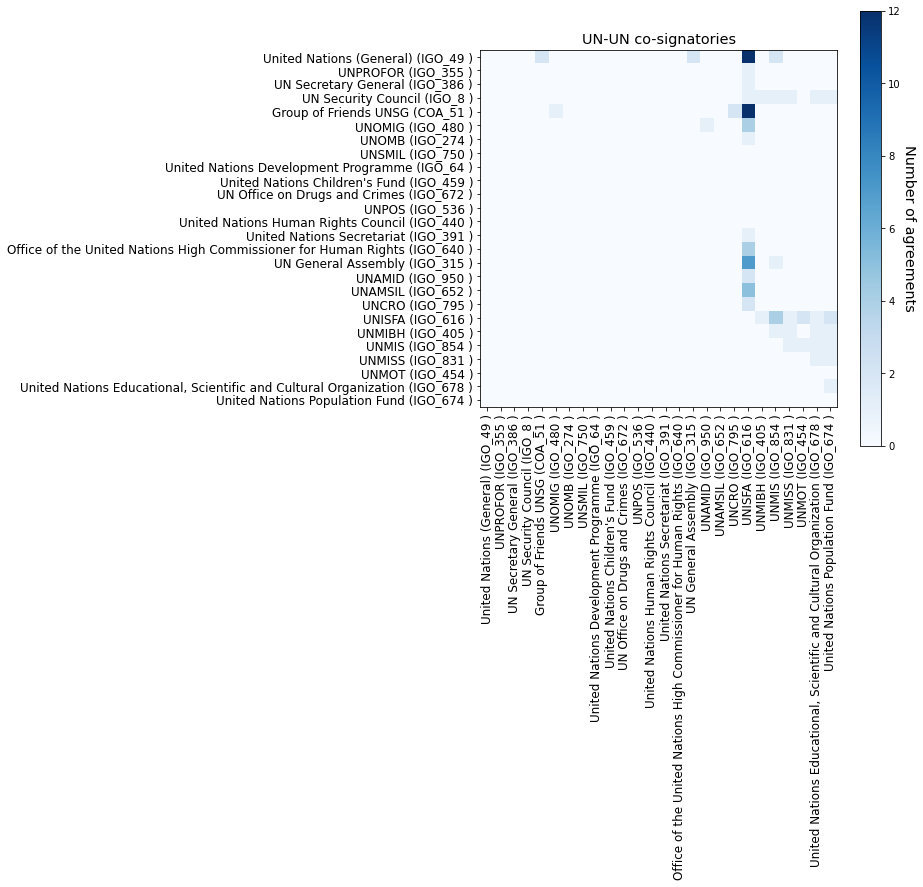
\includegraphics[scale=0.38]{./assets/figure_2.png}
\caption{Heat map showing the number of agreements co-signed by pairs of UN actors. See Table 5 for further information.}
\end{center}
\end{figure}

\begin{figure}[H]
\begin{center}
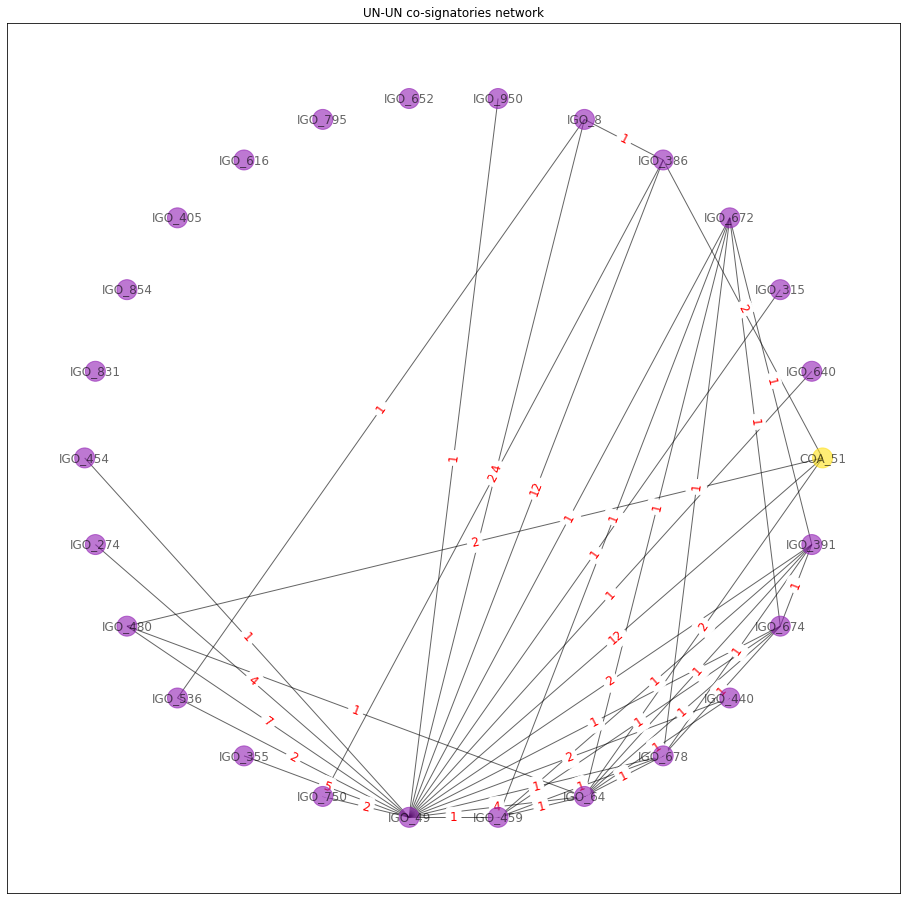
\includegraphics[scale=0.38]{./assets/figure_3.png}
\caption{Network diagram of UN co-signatories. The number of agreements signed by a pair of UN actors is the red number in the connection between the pair. Isolated nodes (known as singletons) are UN actors with no UN co-signatories. See Tables 5 and 6 for further information.}
\end{center}
\end{figure}

\begin{table}[H]
\begin{center}
\small
\begin{tabularx}{\textwidth}{|X|X|r|}
    \hline
    \textbf{Actor 1} & \textbf{Actor 2} & \textbf{Agts} \\
    \hline
    \hline
Group of Friends UNSG (COA\_51) & United Nations (General) (IGO\_49) & 12 \\
\hline
UN Secretary General (IGO\_386) & United Nations (General) (IGO\_49) & 12 \\
\hline
UNOMIG (IGO\_480) & United Nations (General) (IGO\_49) & 7 \\
\hline
UNPROFOR (IGO\_355) & United Nations (General) (IGO\_49) & 5 \\
\hline
UN Security Council (IGO\_8) & United Nations (General) (IGO\_49) & 4 \\
\hline
UNOMB (IGO\_274) & United Nations (General) (IGO\_49) & 4 \\
\hline
United Nations (General) (IGO\_49) & United Nations Development Programme (IGO\_64) & 4 \\
\hline
Group of Friends UNSG (COA\_51) & UN Secretary General (IGO\_386) & 2 \\
\hline
Group of Friends UNSG (COA\_51) & UNOMIG (IGO\_480) & 2 \\
\hline
Group of Friends UNSG (COA\_51) & United Nations Development Programme (IGO\_64) & 2 \\
\hline
UN Secretary General (IGO\_386) & UNSMIL (IGO\_750) & 2 \\
\hline
UNPOS (IGO\_536) & United Nations (General) (IGO\_49) & 2 \\
\hline
UNSMIL (IGO\_750) & United Nations (General) (IGO\_49) & 2 \\
\hline
United Nations (General) (IGO\_49) & United Nations Human Rights Council (IGO\_440) & 2 \\
\hline
United Nations (General) (IGO\_49) & United Nations Secretariat (IGO\_391) & 2 \\
\hline
Office of the United Nations High Commissioner for Human Rights (IGO\_640) & United Nations (General) (IGO\_49) & 1 \\
\hline
UN General Assembly (IGO\_315) & United Nations (General) (IGO\_49) & 1 \\
\hline
UN Office on Drugs and Crimes (IGO\_672) & United Nations (General) (IGO\_49) & 1 \\
\hline
UN Office on Drugs and Crimes (IGO\_672) & United Nations Children's Fund (IGO\_459) & 1 \\
\hline
UN Office on Drugs and Crimes (IGO\_672) & United Nations Development Programme (IGO\_64) & 1 \\
\hline
UN Office on Drugs and Crimes (IGO\_672) & United Nations Educational, Scientific and Cultural Organization (IGO\_678) & 1 \\
\hline
UN Office on Drugs and Crimes (IGO\_672) & United Nations Population Fund (IGO\_674) & 1 \\
\hline
UN Office on Drugs and Crimes (IGO\_672) & United Nations Secretariat (IGO\_391) & 1 \\
\hline
UN Secretary General (IGO\_386) & UN Security Council (IGO\_8) & 1 \\
\hline
UN Security Council (IGO\_8) & UNPOS (IGO\_536) & 1 \\
\hline
UNAMID (IGO\_950) & United Nations (General) (IGO\_49) & 1 \\
\hline
UNMOT (IGO\_454) & United Nations (General) (IGO\_49) & 1 \\
\hline
UNOMIG (IGO\_480) & United Nations Development Programme (IGO\_64) & 1 \\
\hline
United Nations (General) (IGO\_49) & United Nations Children's Fund (IGO\_459) & 1 \\
\hline
United Nations (General) (IGO\_49) & United Nations Educational, Scientific and Cultural Organization (IGO\_678) & 1 \\
\hline
\end{tabularx}
\end{center}
\normalsize
\end{table}


\begin{table}[H]
\begin{center}
\small
\begin{tabularx}{\textwidth}{|X|X|r|}
    \hline
    \textbf{Actor 1 (cont)} & \textbf{Actor 2 (cont)} & \textbf{Agts} \\
    \hline
    \hline
United Nations (General) (IGO\_49) & United Nations Population Fund (IGO\_674) & 1 \\
\hline
United Nations Children's Fund (IGO\_459) & United Nations Development Programme (IGO\_64) & 1 \\
\hline
United Nations Children's Fund (IGO\_459) & United Nations Educational, Scientific and Cultural Organization (IGO\_678) & 1 \\
\hline
United Nations Children's Fund (IGO\_459) & United Nations Population Fund (IGO\_674) & 1 \\
\hline
United Nations Children's Fund (IGO\_459) & United Nations Secretariat (IGO\_391) & 1 \\
\hline
United Nations Development Programme (IGO\_64) & United Nations Educational, Scientific and Cultural Organization (IGO\_678) & 1 \\
\hline
United Nations Development Programme (IGO\_64) & United Nations Human Rights Council (IGO\_440) & 1 \\
\hline
United Nations Development Programme (IGO\_64) & United Nations Population Fund (IGO\_674) & 1 \\
\hline
United Nations Development Programme (IGO\_64) & United Nations Secretariat (IGO\_391) & 1 \\
\hline
United Nations Educational, Scientific and Cultural Organization (IGO\_678) & United Nations Population Fund (IGO\_674) & 1 \\
\hline
United Nations Educational, Scientific and Cultural Organization (IGO\_678) & United Nations Secretariat (IGO\_391) & 1 \\
\hline
United Nations Population Fund (IGO\_674) & United Nations Secretariat (IGO\_391) & 1 \\
\hline
\end{tabularx}
\end{center}
\normalsize
\caption{List of UN actor co-signatories with number of agreements.}
\end{table}

\begin{table}[H]
\begin{center}
\small
\begin{tabularx}{\textwidth}{|X|}
    \hline
    \textbf{UN Actor} \\
    \hline
UNAMSIL (IGO\_652) \\
\hline
UNCRO (IGO\_795) \\
\hline
UNISFA (IGO\_616) \\
\hline
UNMIBH (IGO\_405) \\
\hline
UNMIS (IGO\_854) \\
\hline
UNMISS (IGO\_831) \\
\hline
\end{tabularx}
\end{center}
\normalsize
\caption{UN actors that are not co-signatories with other UN actors.}
\end{table}


\subsection{UN and non-UN co-signatories}

\begin{figure}[H]
\begin{center}
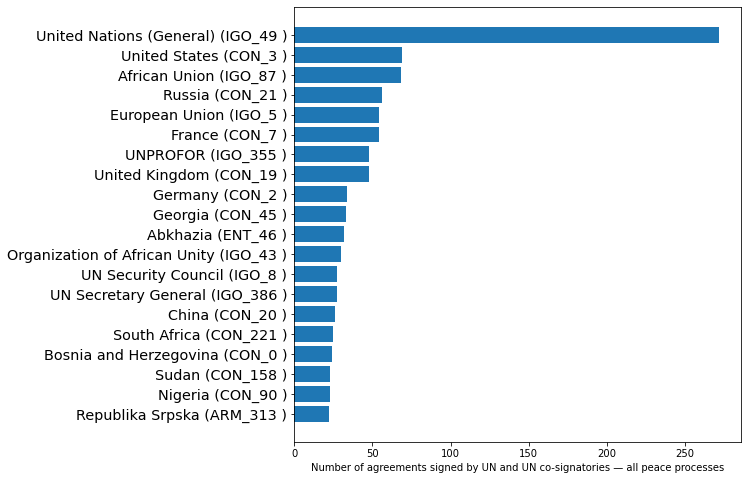
\includegraphics[scale=0.38]{./assets/figure_4.png}
\caption{Number of agreements signed by the top-20 UN and non-UN co-signatories across all peace processes. In total there are 536 actors in the UN--non-UN co-signatory set.}
\end{center}
\end{figure}

\begin{table}[H]
\begin{center}
\small
\begin{tabularx}{\textwidth}{|X|X|r|}
    \hline
    \textbf{UN actor} & \textbf{Non-UN actor} & \textbf{Agts} \\
    \hline
    \hline
United Nations (General) (IGO\_49) & African Union (IGO\_87) & 65 \\
\hline
United Nations (General) (IGO\_49) & United States (CON\_3) & 62 \\
\hline
United Nations (General) (IGO\_49) & European Union (IGO\_5) & 51 \\
\hline
United Nations (General) (IGO\_49) & France (CON\_7) & 47 \\
\hline
United Nations (General) (IGO\_49) & Russia (CON\_21) & 47 \\
\hline
United Nations (General) (IGO\_49) & United Kingdom (CON\_19) & 41 \\
\hline
United Nations (General) (IGO\_49) & Organization of African Unity (IGO\_43) & 30 \\
\hline
United Nations (General) (IGO\_49) & Georgia (CON\_45) & 28 \\
\hline
United Nations (General) (IGO\_49) & Germany (CON\_2) & 28 \\
\hline
United Nations (General) (IGO\_49) & Abkhazia (ENT\_46) & 27 \\
\hline
United Nations (General) (IGO\_49) & South Africa (CON\_221) & 24 \\
\hline
United Nations (General) (IGO\_49) & Sudan (CON\_158) & 22 \\
\hline
United Nations (General) (IGO\_49) & Congo, Democratic Republic of the (CON\_264) & 21 \\
\hline
United Nations (General) (IGO\_49) & Organization for Security and Cooperation in Europe (IGO\_50) & 21 \\
\hline
United Nations (General) (IGO\_49) & Uganda (CON\_176) & 20 \\
\hline
United Nations (General) (IGO\_49) & China (CON\_20) & 20 \\
\hline
United Nations (General) (IGO\_49) & Economic Community of West African States (IGO\_89) & 20 \\
\hline
United Nations (General) (IGO\_49) & Nigeria (CON\_90) & 20 \\
\hline
United Nations (General) (IGO\_49) & Somalia (CON\_358) & 19 \\
\hline
United Nations (General) (IGO\_49) & League of Arab States (IGO\_346) & 19 \\
\hline
United Nations (General) (IGO\_49) & Canada (CON\_11) & 19 \\
\hline
United Nations (General) (IGO\_49) & Norway (CON\_81) & 19 \\
\hline
UNPROFOR (IGO\_355) & Republika Srpska (ARM\_313) & 18 \\
\hline
United Nations (General) (IGO\_49) & Tajikistan (CON\_62) & 18 \\
\hline
United Nations (General) (IGO\_49) & Kenya (CON\_172) & 18 \\
\hline
United Nations (General) (IGO\_49) & Italy (CON\_139) & 17 \\
\hline
United Nations (General) (IGO\_49) & Guatemala  (CON\_306) & 17 \\
\hline
UNPROFOR (IGO\_355) & Bosnia and Herzegovina (CON\_0) & 16 \\
\hline
United Nations (General) (IGO\_49) & Guatemalan National Revolutionary Unity (ARM\_307) & 15 \\
\hline
United Nations (General) (IGO\_49) & Organisation of Islamic Cooperation (IGO\_226) & 15 \\
\hline
\end{tabularx}
\end{center}
\normalsize
\caption{Top-30 UN--non-UN co-signatory pairings with number of agreements in common. The total number of UN--non-UN actor pairings is 1287.}
\end{table}

\pagebreak

\begin{table}[H]
\begin{center}
\small
\begin{tabularx}{\textwidth}{|X|X|r|}
    \hline
    \textbf{UN actor} & \textbf{Non-UN actor} & \textbf{Agts} \\
    \hline
    \hline
UNSMIL (IGO\_750) & Switzerland (CON\_202) & 1 \\
\hline
UNSMIL (IGO\_750) & Libyan Army (MIL\_941) & 1 \\
\hline
UNSMIL (IGO\_750) & Tunisia (CON\_590) & 1 \\
\hline
UNSMIL (IGO\_750) & Turkey (CON\_562) & 1 \\
\hline
UNSMIL (IGO\_750) & Germany (CON\_2) & 1 \\
\hline
United Nations Human Rights Council (IGO\_440) & Liberia (CON\_83) & 1 \\
\hline
United Nations Human Rights Council (IGO\_440) & Mali (CON\_93) & 1 \\
\hline
United Nations Human Rights Council (IGO\_440) & International Committee of the Red Cross (NGO\_201) & 1 \\
\hline
United Nations Human Rights Council (IGO\_440) & Côte d’Ivoire (CON\_88) & 1 \\
\hline
United Nations Human Rights Council (IGO\_440) & Togo (CON\_85) & 1 \\
\hline
United Nations Human Rights Council (IGO\_440) & Cape Verde (CON\_354) & 1 \\
\hline
United Nations Human Rights Council (IGO\_440) & International Monetary Fund (IGO\_438) & 1 \\
\hline
United Nations Human Rights Council (IGO\_440) & Niger (CON\_142) & 1 \\
\hline
United Nations Human Rights Council (IGO\_440) & Nigeria (CON\_90) & 1 \\
\hline
United Nations Human Rights Council (IGO\_440) & High Commission for Refugees (IGO\_65) & 1 \\
\hline
\end{tabularx}
\end{center}
\normalsize
\caption{Bottom-15 UN--non-UN co-signatory pairings with number of agreements in common. The total number of UN--non-UN actor pairings is 1287.}
\end{table}

\pagebreak

\section{Case Study: United Nations (General) }

The analysis described below can be applied to any actor.

Analysis by:

\begin{itemize}
\item Co-signatories
\item Agreements with co-signatories (top-n)
\item Year - time series
\item Peace Process
\item Agreement stage
\item Other metadata (region?)
\end{itemize}
 

\end{document}
















